\documentclass{thesis}
% Damit die Verwendung der deutschen Sprache nicht ganz so umst\"andlich wird,
% sollte man die folgenden Pakete einbinden: 
\usepackage[latin1]{inputenc}% erm\"oglich die direkte Eingabe der Umlaute 
\usepackage[T1]{fontenc} % das Trennen der Umlaute
\usepackage{cite}
\usepackage{graphicx}
\usepackage{subfig}
\usepackage{caption}
\usepackage{amssymb,amsmath}
%\def\BibTeX{{\rm B\kern-.05em{\sc i\kern-.025em b}\kern-.08em
 %   T\kern-.1667em\lower.7ex\hbox{E}\kern-.125emX}}
\usepackage[german,german]{babel} % hiermit werden deutsche Bezeichnungen genutzt und 
                     % die W\"orter werden anhand der neue Rechtschreibung 
		     % automatisch getrennt.  
\title{Trapping and Beamloading in hybrid Plasma Wakefield Accelerator schemes}
\author{Alexander Knetsch}

\date{\today}
% Hinweis: \title{um was auch immer es geht}, \author{wer es auch immer 
% geschrieben hat} und  \date{wann auch immer das war} k\"onnen vor 
% oder nach dem  Kommando \begin{document} stehen 
% Aber der \maketitle Befehl mu\ss{} nach dem \begin{document} Kommando stehen! 
% TEst3
\begin{document}

\maketitle
\tableofcontents

\begin{figure}
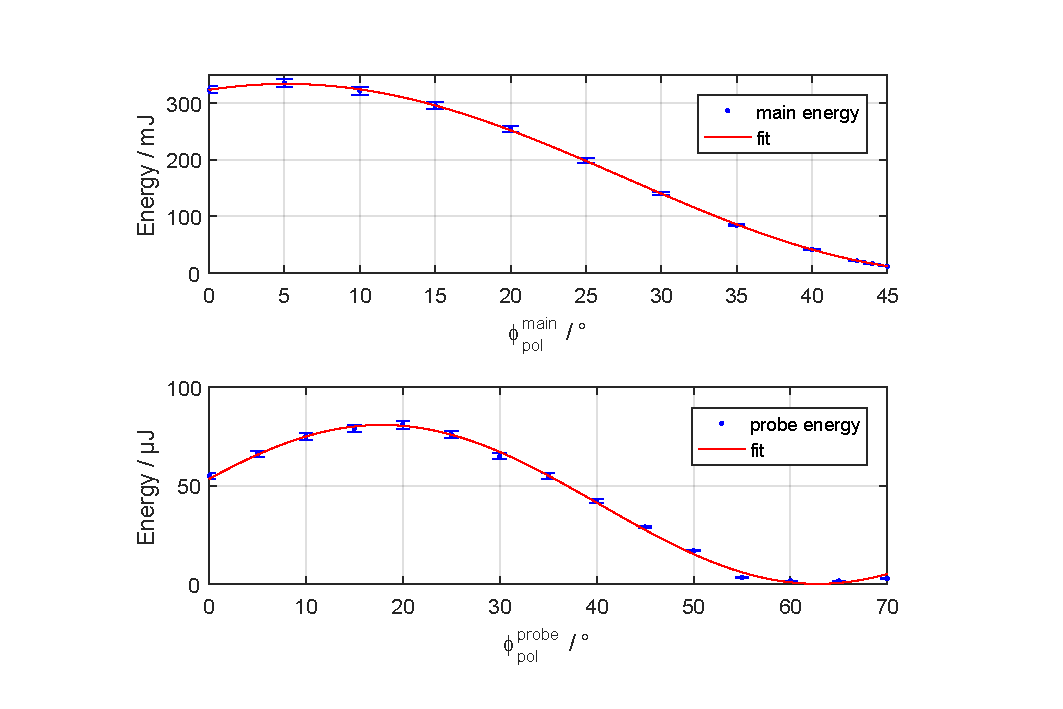
\includegraphics[width=1.0\textwidth]{experiment/images/raw/waveplate_calibration.pdf}
\end{figure}


$$I=\hat{I}_{x,y}W_\mathrm{Laser}/(2\sqrt{\pi}\sigma_t(\Delta x_\mathrm{res}\times10^-6)^2)$$
In order to derive an expression for the trapping condition of a single electron in PWFA, one has to start with the equation of motion for such a single electron. 
\begin{equation}
F=\frac{d\vec{p}}{dt}=q(\vec{E}\times \vec{B})
\end{equation}
with the electron charge $q$ electric field $\vec{E}$ and magnetic field $\vec{B}$


This leads to the single particle electron hamiltonian. 
\begin{align}
\frac{dH}{dt}&=\frac{d}{dt} (\gamma m_e c^2)+\frac{d}{dt}(q\Phi)\\
&=\vec{v}\frac{d\vec{p}}{dt}+\frac{d}{dt}(q\Phi)\\
&=q\vec{v}(-\nabla \Phi-\frac{\partial \vec{A}}{\partial t})+\frac{\vec{v}\times\vec{B}}{c}+\frac{d}{dt}(q\Phi)\\
&=q(\frac{d}{dt}\Phi-\vec{v}\vec{\nabla}\Phi-\vec{v}\frac{\partial \vec{A}}{\partial t})\\
&=q(\frac{\partial \Phi}{\partial t}-\vec{v}\frac{\partial \vec{A}}{\partial t})
\end{align}

If one assumes now, that the wake fields are constant during the trapping process, then 

\begin{align}
H-v_\mathrm{\phi}P_z &= \mathrm{const.}\\
\gamma m c^2+\Psi-v_\mathrm{\phi}p_z-v_\mathrm{\phi}qA_z &= \mathrm{const.}\\
\gamma+\frac{q \Phi}{m c^2}-v_\mathrm{\phi} \frac{p_z}{mc^2} &= \mathrm{const.}\\
\gamma - v_\mathrm{\phi} \frac{p_z}{mc^2} \underbrace{\frac{q}{mc^2}(\Phi-v_\mathrm{\phi}A_z)}_{\hat{\Psi}}  &= \mathrm{const.} 
\end{align}
%- \underbrace{\frac{q}{mc^2}(\Phi-v_\mathrm{\phi}A_z)}_

which is especially true for the hamiltonian.
\begin{align*}
\frac{d}{dt}H&=q(\frac{\partial \Phi}{\partial t}-\vec{v}\frac{\partial \vec{A}}{\partial t})\\
&=-q v_\mathrm{\phi}(\frac{\partial \Phi}{\partial z}-\vec{v} \frac{\partial \vec{A}}{\partial z})
\end{align*}
The trapping of a single electron in PWFA happens in a short time (i.e. a short propagation distance) compared to the timescales on which the wakefield changes its shape. An example for a distance over which the wakefield is modified is the betatron length FORUMLA !!!.
This gives the convenient possibility to treat the problem in a frame moving along with the phase velocity of the wake $v_\phi$. Mathematically this can be done by finding a constant $C_\mathrm{H}$ with $\frac{d C_\mathrm{H}}{dt}=0$ , so that $\frac{d}{dt}(H-C_\mathrm{H})=0$.
W. Lu suggested in his thesis [citation needed !!!] 
\begin{align*}
\frac{d}{dt}(H-v_\mathrm{\phi} P_z)&=-qv_\mathrm{\phi}(\frac{\partial \Phi}{\partial z}-\vec{v}\frac{\partial \vec{A}}{\partial z})-qv_\mathrm{\phi}(v_z \frac{\partial A_z}{\partial z}-\frac{\partial \Phi}{\partial z})\\
&\approx q v_\mathrm{\phi}(v_z \frac{\partial A_z}{\partial z}-v_z \frac{\partial A_z}{\partial z})=0
\end{align*}

\begin{align*}
H-v_\mathrm{\phi}P_z&=const.\\
\gamma m c^2+q\Phi-v_\mathrm{\phi}p_z-v_\mathrm{\phi}qA_z&=const.\\
\gamma+\frac{q\Phi}{mc^2}-v_\mathrm{\phi}\frac{p_z}{mc^2}-v_\mathrm{\phi}q\frac{A_z}{mc^2}&=const\\
\gamma-v_\mathrm{\phi}\frac{p_z}{mc^2}-\underbrace{\frac{q}{mc^2}(\Phi-v_\mathrm{\phi}A_z)}_{\Psi}&=const.\\
-const. +\gamma + v_\mathrm{\phi}\frac{p_z}{mc^2}&=\Psi
\end{align*}

\begin{align*}
\Psi_f-\Psi_i=\gamma_f-\gamma_i-v_\mathrm{\phi}\frac{\gamma_f m v_f}{mc^2}
\end{align*}

\begin{align*}
Q'(z)=\int_{-\infty}^{\infty}1- exp(W_\mathrm{ADK}(z,t))\ dt
\end{align*}


\bibliography{lib}
\bibliographystyle{plain}    
\end{document}